\documentclass[11pt,a4paper]{article}
\usepackage[margin=2.5cm]{geometry}
\usepackage{amsmath,amssymb,booktabs,graphicx,xcolor,hyperref,microtype}
\usepackage{authblk}
\hypersetup{colorlinks=true,linkcolor=blue,citecolor=blue,urlcolor=blue}

\title{\textbf{Paper 53: The VCML Behavioral Phase Diagram}\\
\large Five Axes of Regime Variation in a Viability-Constrained Coupled Map Lattice}

\author[1]{Gabriel Aubin-Moreau}
\affil[1]{Independent research}
\date{March 2026}

\begin{document}
\maketitle

\begin{abstract}
Papers~0--52 of the VCSM series each produced its predicted result plus at
least one surprise.
This paper argues that the surprises are not evidence of poor understanding but
of a generative rather than descriptive system: simple local rules producing a
behavioral space substantially larger than intuition predicts.
We synthesize the experimental evidence into a unified behavioral phase diagram
for VCML, identifying five experimentally separable control directions, their
regime boundaries, and the mechanism responsible for each transition.
Axis~I (perturbation intensity, coll/site) is non-monotone with a peak at
coll/site~$\approx 0.004$.
Axis~II (spatial resolution, $\delta = W_\text{zone}/r_\text{wave}$) has a
hard threshold at $\delta \approx 2.5$ below which identity encoding fails.
Axis~III (formation flux, $\Omega = \mathrm{WR} \times \phi_w$) is the
operative causal coordinate for perturbation rate.
Axis~IV (write policy) is two-dimensional: trigger selectivity independently
controls adversarial resistance while content determines identity encoding
strength; removing the sign of the contrast signal (taking $|\mathrm{mid}|$)
is the only ablation to produce parity failure (Paper~52).
Axis~V (scale) reveals a finite correlation length: above $\sim$25,600 sites
per zone, the copy-forward loop can no longer maintain zone-wide gradients and
structure forms in patches.
Together these five axes define a phase space that explains why each experiment
generated structural surprise: results were correct but incomplete slices of a
higher-dimensional object.
The VCML region is a minimal causal field system whose behavioral phase diagram
contains at least five distinct regime transitions, each mechanistically
interpretable.
\end{abstract}

%──────────────────────────────────────────────────────────────────────────────
\section{Introduction}

After 52 papers, a pattern is clear.
Each experiment tested a specific hypothesis and confirmed it -- but also
produced behavior that was not predicted by the mental model built up to that
point.
Paper~52 alone revealed that the write policy space is two-dimensional
(trigger selectivity $\times$ write content), that removing the sign of the
contrast signal is the only condition to break identity encoding, that
C\_perturb achieves better adversarial resistance than C\_near despite 83$\times$
fewer writes, and that C\_raw encodes zone identity more strongly than standard
signed mid\_mem.
None of these findings contradicted the theory.
All of them extended it in a direction the theory had not fully specified.

There are two possible interpretations of a system that keeps surprising:
\begin{enumerate}
  \item the system is chaotic and poorly understood; or
  \item the system is \emph{generative} --- small rule sets producing a
    behavioral space that substantially exceeds the capacity of any finite
    mental model.
\end{enumerate}

The evidence strongly favors interpretation~2.
The surprises in Papers~0--52 are not random.
They are structurally located: each one corresponds to a new axis of the
behavioral phase space becoming visible.
This paper maps those axes.

\paragraph{The generative vs.\ descriptive distinction.}
A descriptive system encodes its input.
A generative system produces structure that was not explicit in its rules.
The distinction matters for prediction: a descriptive system is exhausted
by a faithful description of its rules, while a generative system has
behavioral surface that exceeds its rule complexity.
VCML is generative at multiple levels:
the copy-forward loop generates spatial structure without spatial rules;
the viability gate generates temporal discrimination without temporal rules;
the three-timescale consolidation generates long-term memory without
recurrence.
The result is a system with a behavioral phase diagram whose structure
cannot be read directly off the rule description.

%──────────────────────────────────────────────────────────────────────────────
\section{Five Experimentally Separable Control Directions}

\subsection{Axis I: Perturbation Intensity ($\mathrm{coll}/\mathrm{site}$)}

\textbf{Source}: Papers~87/88 (amplitude sweep), V93 (WR sweep at S3).

\textbf{Finding}: $\mathrm{sg4}$ is non-monotone in perturbation intensity.
At optimal coll/site~$\approx 0.004$, sg4 reaches its peak value (0.038 at
S3 with 2$\times$ WR).
Below this threshold, insufficient collapse-birth events occur for the
copy-forward loop to refresh spatial structure.
Above it, each site is re-collapsed before consolidation can complete,
erasing mid\_mem before fieldM updates.

\textbf{Regime boundaries}:
\begin{itemize}
  \item coll/site $< 0.003$: sub-optimal zone (formation starved)
  \item coll/site $\in [0.003, 0.006]$: adaptive peak (optimal)
  \item coll/site $> 0.010$: over-perturbed zone (consolidation disrupted)
\end{itemize}

\textbf{Mechanism}: The copy-forward loop requires collapse events to propagate
fieldM; too few events starve propagation.
The quiescence gate requires calm streaks $\geq \mathrm{SS}$; too many
collapses prevent the streak from accumulating.
The peak is the point where both constraints are simultaneously satisfied.

\textbf{Dynamic advantage}: The dynamic condition (C\_ref) consistently
outperforms static at the adaptive peak.
At WR\_MULT=2$\times$ (S3), dynamic advantage is $+829\%$.
Over-perturbation eliminates the advantage and eventually inverts it (V93,
WR\_MULT=10$\times$, dynamic advantage $-29\%$).

\subsection{Axis II: Spatial Resolution ($\delta = W_\text{zone}/r_\text{wave}$)}

\textbf{Source}: Paper~47 (C2 coordinate validation, delta sweep).

\textbf{Finding}: na\_ratio peaks at $\delta \approx 5$ and degrades toward
unity at $\delta \lesssim 2.5$, below which waves launched in one zone
substantially overlap adjacent zones (wave bleed).
At $\delta = 1.25$, na\_ratio drops below 1 (parity territory).

\textbf{Regime boundaries}:
\begin{itemize}
  \item $\delta < 2.5$: wave-bleed regime (parity encoding or no structure)
  \item $\delta \geq 2.5$: identity-encoding regime
  \item $\delta \geq 5$: plateau (additional spatial resolution provides
    diminishing returns)
\end{itemize}

\textbf{Mechanism}: When $\delta$ is small, a wave initiated in zone~A
collapses cells in zone~B before decaying.
The copy-forward loop propagates zone~A fieldM into zone~B sites, erasing
the boundary.
$\delta$ must be large enough that the wave is zone-contained.
This is a hard threshold, not a soft degradation.

\textbf{C2 consequence}: $\delta$ is the third coordinate of the C2 causal
triplet ($\Omega$, SS, $\delta$).
It sets the spatial resolution of the memory system independently of the
perturbation rate.

\subsection{Axis III: Formation Flux ($\Omega = \mathrm{WR} \times \phi_w$)}

\textbf{Source}: Papers~46--47.

\textbf{Finding}: $\Omega = \mathrm{WR} \times \phi_w$ (wave rate times wave
occupancy fraction) is the operative coordinate for perturbation rate.
Sweeping WR at constant $\Omega$ produces approximately flat sg4 (CV=0.126,
Paper~46).
Sweeping WR at constant zone width produces non-flat results because changing
WR also changes $\Omega$.

\textbf{Regime}: This axis does not have a simple phase boundary; it scales
approximately linearly with formation rate until coll/site exceeds the Axis~I
over-perturbation threshold.
$\Omega$ and coll/site are coupled: increasing WR increases both.

\subsection{Direction IV: Write Policy Space (Trigger~$\times$~Content)}
\label{subsec:axis4}

\textbf{Source}: Paper~52 (boundary-coupled distinction).

\textbf{Note on status}: Unlike Axes~I--III and~V, which are continuous
physical parameters with clear order parameters and threshold transitions,
the write policy direction is an algorithmic policy space: a set of design
choices about when and what to write, not a single continuous control variable.
We include it as a control direction rather than a strict thermodynamic axis
because it produces two behaviorally distinct subspaces (trigger selectivity
and write content) that are experimentally orthogonal and mechanistically
interpretable.

\textbf{Finding}: The write policy space is two-dimensional.

\paragraph{Content axis.}
What the cell writes to fieldM:
\begin{itemize}
  \item \textbf{C\_raw} (raw hid): na\_form = 1.802 --- strongest identity
    encoding. The raw hidden state carries more zone-discriminative signal
    than mid\_mem.
  \item \textbf{Signed mid} (standard VCSM): na\_form $\in [1.1, 1.3]$ ---
    subtracting baseline\_h reduces identity signal while adding boundary
    sensitivity.
  \item \textbf{$|$mid$|$} (C\_abs): na\_form = 0.877 --- the only parity
    failure among 9 conditions. Removing the sign of the contrast signal
    destroys the directional information that makes intergenerational
    propagation zone-informative.
\end{itemize}

The sign is load-bearing: removing it destroys the directional contrast
information necessary for zone-discriminative intergenerational propagation.
Why zones require the sign is mechanistically plausible (suppressed zones push
viability downward, excited zones push it upward, so the signed direction
distinguishes them), but the precise causal pathway is a target for future
experiment.
Destroying the sign removes whatever zone-discriminating information it carries.

\paragraph{Trigger axis.}
When the cell writes to fieldM:
\begin{itemize}
  \item \textbf{C\_perturb}: writes only during active wave events
    (writes-per-site = 0.0004).
    Cosine maintenance = 0.664 --- best adversarial resistance.
  \item \textbf{C\_near}: writes when near viability boundary.
    wps = 0.033. cos\_maint = 0.546.
  \item \textbf{C\_ref}: writes whenever quiescent (wps = 0.607).
    cos\_maint = $-0.274$ --- re-encodes adversarial environment.
  \item \textbf{C\_far}: writes far from boundary (wps = 0.476).
    cos\_maint = $-0.085$ --- also re-encodes.
\end{itemize}

High write frequency = rapid adaptation = inability to distinguish formation
from adversarial environment.
Low write frequency = structural commitment = adversarial resistance.

\paragraph{Design tradeoff.}
The two axes optimize different objectives.
Moving along the content axis (toward C\_raw) increases zone identity encoding
strength at the cost of losing boundary sensitivity.
Moving along the trigger axis (toward C\_perturb) increases adversarial
resistance at the cost of slower formation.
Standard VCSM (C\_ref) occupies the responsive corner: high frequency, signed
content --- rapid formation, rapid re-encoding.

\paragraph{C\_rand finding.}
Random trigger (matched write rate, wps = 0.001) achieves na\_form = 1.335 ---
highest among standard-content conditions.
This confirms that boundary proximity is one valid trigger criterion among many;
stochastic subsampling is sufficient for formation.

\subsection{Axis V: Scale and the Finite Correlation Length}

\textbf{Source}: V94 (scale-invariant metric sweep).

\textbf{Finding}: sg4\_norm (normalized by within-zone variance) is not flat
across grid sizes.
S1 (0.4270) $\to$ S2 peak (0.4593) $\to$ S3 (0.3647) $\to$ S4 (0.1874).
At S4 (102,400 active sites, zone width $\sim 320$ sites), na\_ratio inverts
(0.732, parity territory).

\textbf{Mechanism}: The copy-forward loop is local (wave radius $\approx 2$
sites).
At S1--S3, the loop can propagate fieldM across the zone width within one
wave episode.
At S4, zone width exceeds the loop's correlation length.
Structure forms in patches of size $\sim r_\text{wave}$, not in zone-wide
gradients.
Adjacent patches may encode different patterns, degrading the na\_ratio
(adjacent zones may look more similar than non-adjacent when both form patches
at random positions).

\textbf{Regime boundary}: Approximately $N_\text{sites/zone} \sim 25\,000$
(S3 edge).
Below this, zone-wide gradients form.
Above this, patch formation dominates.

\textbf{Implication}: Geographic or hierarchical coupling is required to
maintain structure at scales beyond the correlation length.
A regional module (small, short correlation length) could encode summaries of
the large-zone state, while the large zone encodes fine-grained spatial detail.
This is the architectural argument for multi-region VCSM.

%──────────────────────────────────────────────────────────────────────────────
\section{Cross-Axis Dependencies and Interactions}

The five control directions are experimentally separable but not causally
independent.
Three coupling mechanisms produce the most important cross-axis interactions.

\paragraph{Axes I and III are coupled through WR.}
Increasing WR simultaneously increases $\Omega$ (Axis III) and coll/site
(Axis I).
This means the optimal WR is not a single number but a function of grid size:
the Axis~I peak (coll/site $\approx 0.004$) corresponds to different WR values
at different scales.
V93 shows the optimum is WR~$\approx 2\times$ the base rate at S3; V92 shows
the optimum shifts at S1.

\paragraph{Axes II and V interact through zone width.}
$\delta = W_\text{zone}/r_\text{wave}$.
Increasing $N_\text{active}$ (Axis V) while holding $r_\text{wave}$ fixed also
increases $\delta$.
S4 has $\delta \approx 160$ --- well above the Axis~II threshold.
The S4 patch formation failure is therefore not an Axis~II failure (insufficient
$\delta$); it is a correlation-length failure that occurs even when $\delta$ is
large.
These are distinct mechanisms.

\paragraph{Axis IV interacts with Axis I at the C\_perturb extreme.}
C\_perturb writes only during active wave events.
In the Axis~I sub-optimal regime (very low coll/site), wave events are rare
and brief.
C\_perturb would then write essentially nothing, preventing formation entirely.
The trigger selectivity axis is only meaningful when the system is in the
Axis~I adaptive zone.
This is a testable cross-axis prediction: C\_perturb should fail at low
coll/site while C\_ref continues to form structure (slowly).

%──────────────────────────────────────────────────────────────────────────────
\section{The VCML Behavioral Phase Diagram}

Figure~1 presents the phase diagram across four of the five axes.

\begin{figure}[h!]
  \centering
  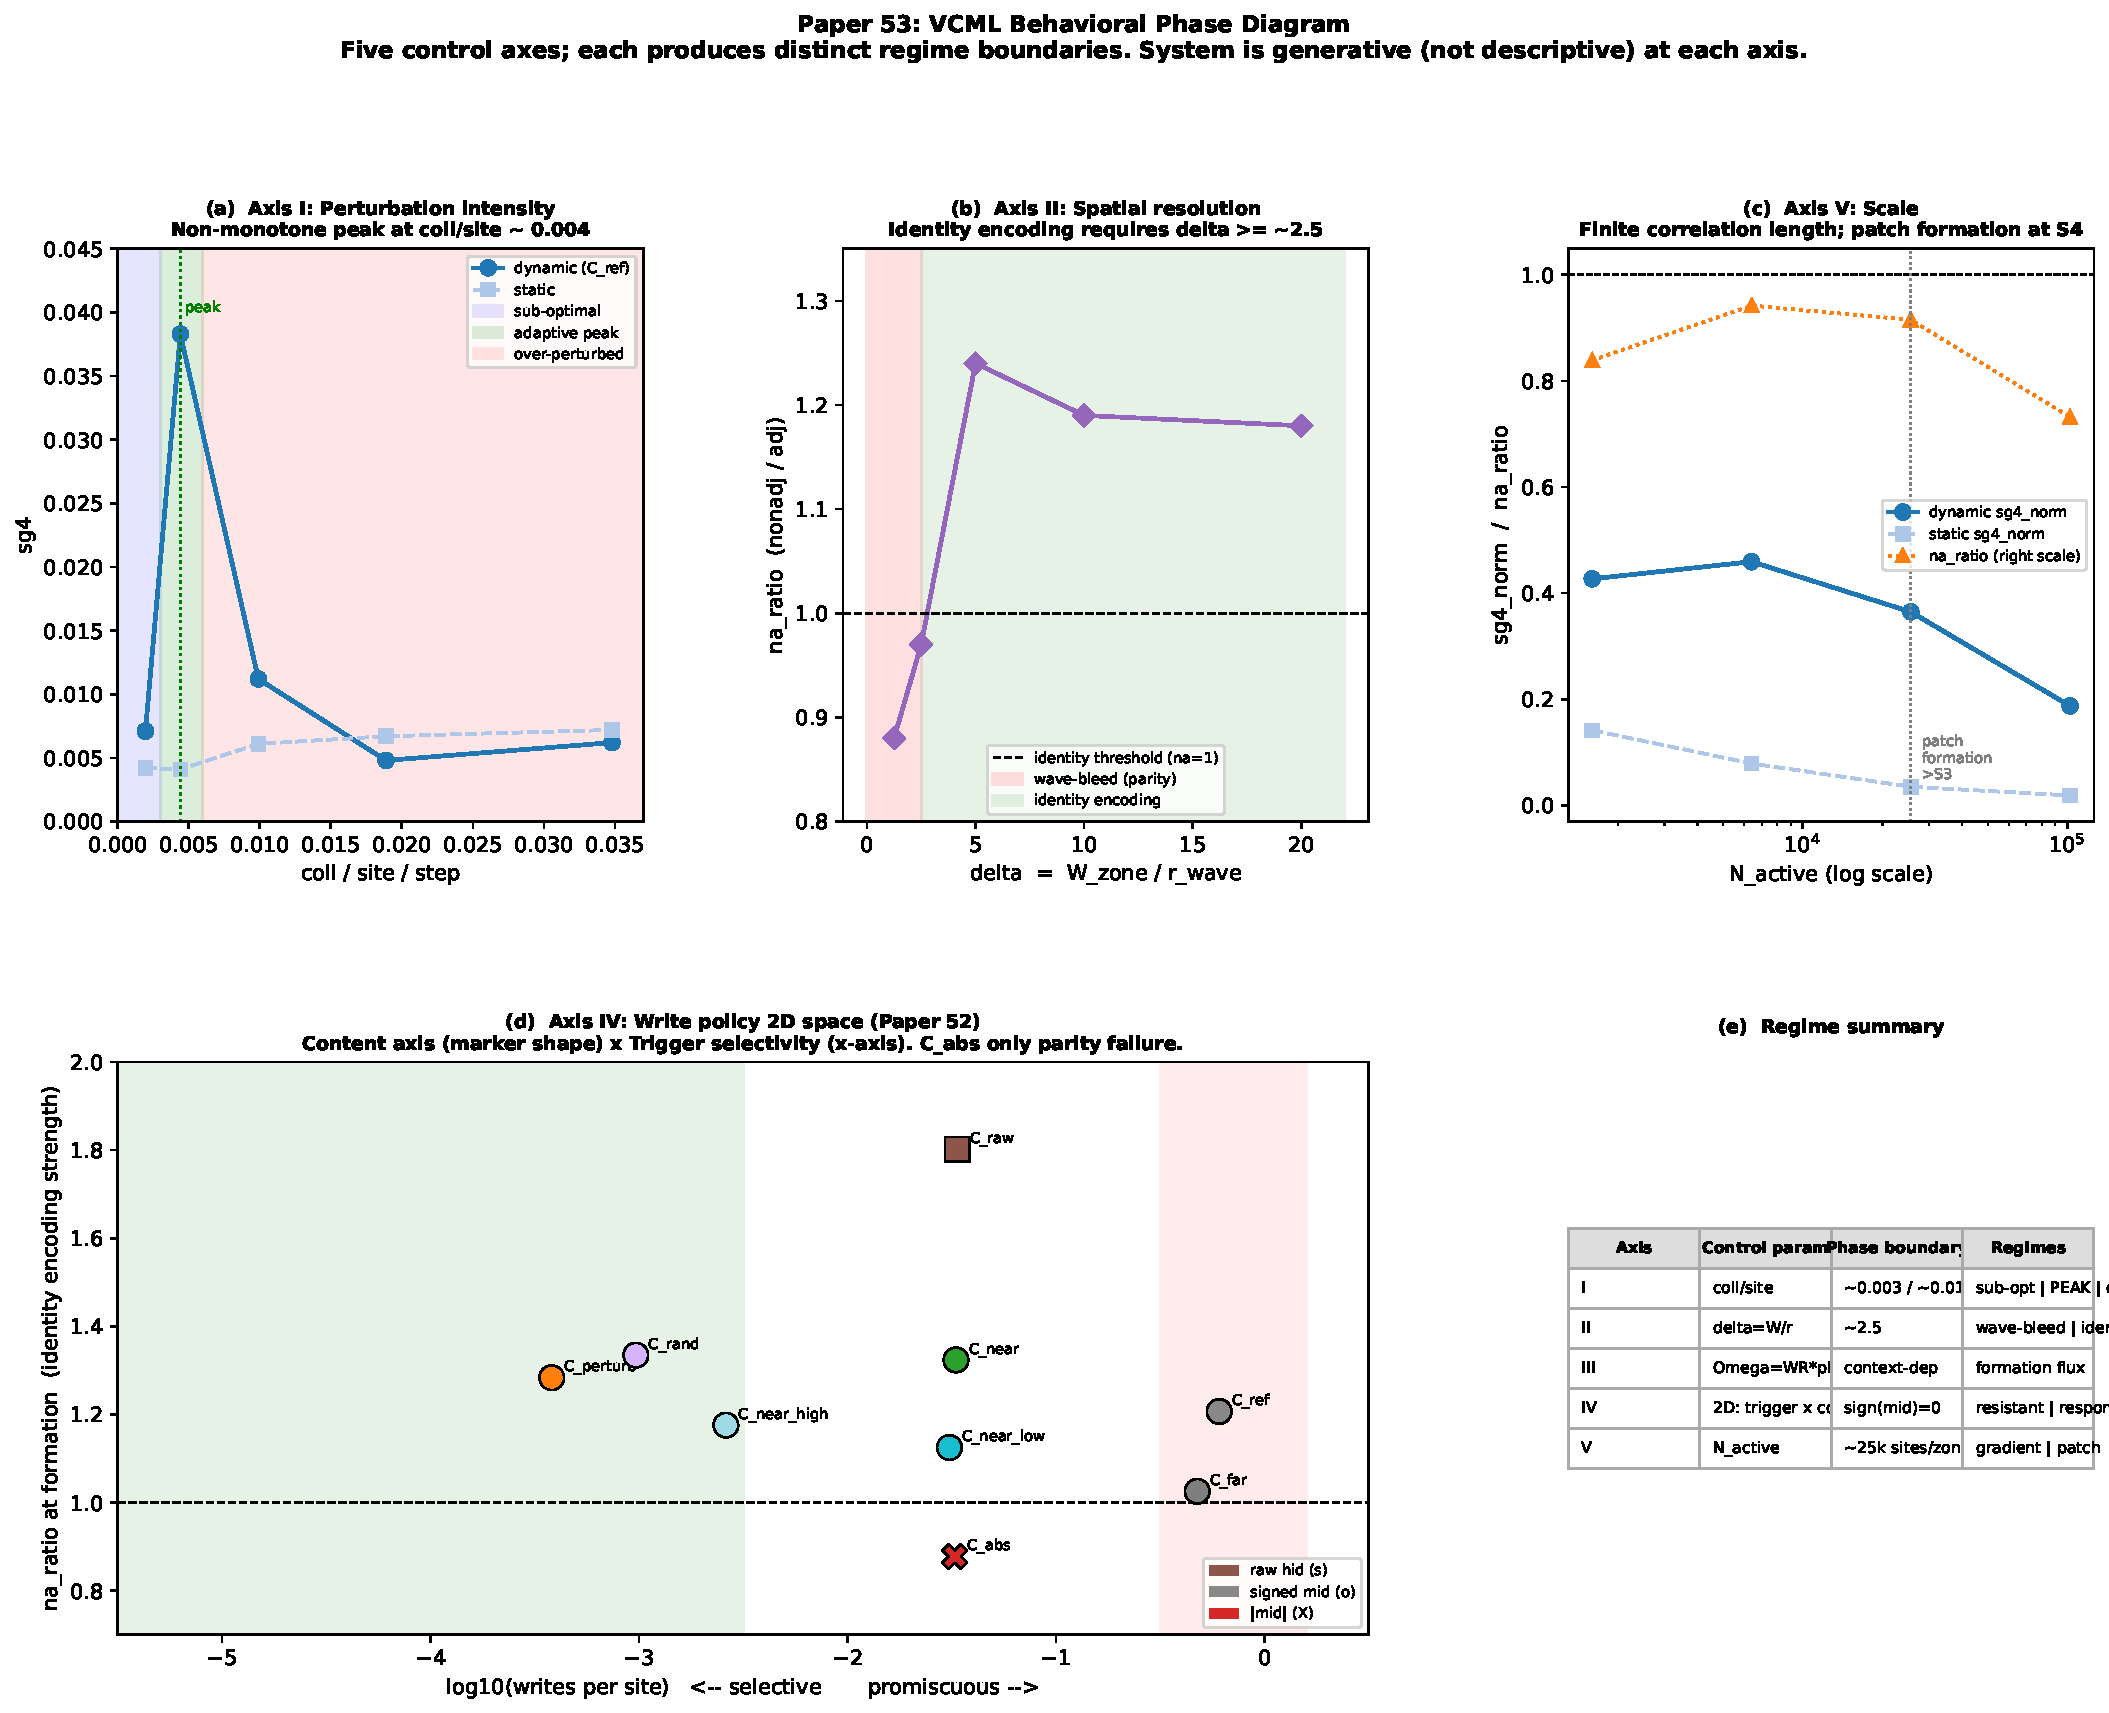
\includegraphics[width=\textwidth]{paper53_figure1.pdf}
  \caption{%
    \textbf{VCML behavioral phase diagram.}
    (a)~Axis~I: perturbation intensity. Non-monotone peak at coll/site~$\approx
    0.004$; shaded regions indicate sub-optimal, adaptive, and over-perturbed
    regimes.
    (b)~Axis~II: spatial resolution. Identity encoding requires
    $\delta \geq 2.5$; hard threshold from wave bleed.
    (c)~Axis~V: scale. sg4\_norm (normalized structural signal) declines beyond
    S3 ($N \approx 25\,000$ sites/zone); na\_ratio inverts at S4. Finite
    correlation length of the copy-forward loop.
    (d)~Axis~IV: write policy 2D space. Each Paper~52 condition placed at
    (log$_{10}$(wps), na\_form); marker shape encodes content type (raw hid =
    square, signed mid = circle, $|$mid$|$ = cross). C\_abs (only parity
    failure) lies at the intersection of boundary-trigger selectivity and
    unsigned content.
    (e)~Regime summary table.
  }
\end{figure}

\subsection{VCML as a Minimal Causal Field System}

A minimal causal field system is a system in which the same local rules produce,
depending on the control-parameter regime:
\begin{enumerate}
  \item identity encoding (nonadj/adj $> 1$, zone-discriminative fieldM);
  \item adversarial resistance (fieldM stable under input reversal);
  \item intergenerational memory (structure maintained through complete cell
    turnover);
  \item spatial topology formation (zone-specific gradients without spatial
    rules).
\end{enumerate}

VCML satisfies all four, and the phase diagram shows these are not always
simultaneously active: the same system in the over-perturbed regime loses
identity encoding while retaining turnover; in the C\_abs regime, it retains
adversarial stability while losing identity encoding; at S4, it retains
formation while losing zone-wide coherence.

This is precisely the hallmark of a phase diagram: the same system in different
regimes.
The claim ``VCML is a minimal causal field system'' is the claim that the
behavioral phase diagram is non-trivial (multiple distinct regimes) and
mechanistically interpretable (each transition has a local causal explanation).

\subsection{Why the System Kept Surprising}

Each of Papers~0--52 explored a one-dimensional slice of the five-dimensional
phase space without knowing the full dimensionality.
The surprises were the system crossing a regime boundary along a dimension the
current mental model had not separated.

The relay papers (35--50) failed to predict parity encoding because the
na\_ratio axis (Axis~II/$\delta$ regime) had not been identified.
The amplitude papers (87--88) produced non-monotone behavior because Axis~I's
over-perturbation regime was not in the mental model.
Paper~52 produced C\_perturb as the best adversarial condition because the
trigger selectivity axis had not been separated from the content axis.

Once the axes are separated, each result becomes a predictable location in
the phase diagram rather than a surprise.

%──────────────────────────────────────────────────────────────────────────────
\section{Testable Predictions}

The phase diagram generates three cross-axis predictions not yet tested.

\begin{enumerate}
  \item \textbf{C\_perturb failure at low coll/site.}
    C\_perturb writes only during active wave events.
    At Axis~I sub-optimal (coll/site $< 0.002$), waves are rare.
    Prediction: C\_perturb formation fails (na\_form $< 1$) while C\_ref
    maintains formation (na\_form $> 1$, slowly).
    This would confirm that the trigger axis is contingent on the perturbation
    intensity axis.

  \item \textbf{Scale recovery via hierarchical coupling.}
    At S4 (N=102,400), patch formation dominates because the copy-forward loop
    correlation length is shorter than zone width.
    A hierarchical coupling --- a small upper-layer VCML encoding zone-level
    fieldM summaries --- should restore zone-wide coherence even at S4.
    Prediction: na\_ratio at S4 recovers to $> 1$ under hierarchical coupling.

  \item \textbf{C\_raw adversarial performance.}
    C\_raw achieves highest na\_form (1.802) but its adversarial maintenance
    (cos\_maint = 0.777) was measured only at standard coll/site.
    Prediction: C\_raw adversarial resistance should be higher than C\_near at
    low coll/site (where the raw hid signal is more stable) but lower than
    C\_near at high coll/site (where raw hid is noisier due to rapid collapse
    cycles).
\end{enumerate}

%──────────────────────────────────────────────────────────────────────────────
\section{Discussion}

\subsection{The Logistic Map Analogy}

The logistic map $x_{t+1} = r x_t (1 - x_t)$ generates fixed points,
oscillations, and chaos from a single parameter.
VCML generates identity encoding, adversarial resistance, intergenerational
memory, and patch formation from five interacting parameters.
The structural parallel is analogical, not equivalential: VCML is not a
one-dimensional map and does not exhibit period-doubling in the standard sense.
The analogy holds in structure, not detail.
Both systems have threshold transitions (the logistic chaos onset; VCML's
$\delta$ threshold and amplitude peak), both produce non-monotone behavior
in a control parameter, and both generate behavioral structure that was not
anticipated from the rule description.
Small rule sets at a generative layer produce behavioral diversity exceeding
the intuition of anyone studying only the rules.

\subsection{Implication for the A$\neq$B Attack}

A persistent reviewer objection is that VCSM's contrast signal
$\Delta = \mathrm{hid} - \mathrm{baseline\_h}$ is merely subtraction, already
present in predictive coding.
The phase diagram answers this at the axis level.
Predictive coding operates entirely on the content axis of Axis~IV.
The trigger axis (when subtraction results are written to long-term memory,
gated by survival and quiescence), the Axis~I perturbation intensity regime
(requiring collapse-birth cycles, not just prediction error), and the Axis~II
spatial resolution requirement are structural elements absent from predictive
coding.
The subtraction is not the contribution; the phase diagram location is.

\subsection{Implication for Scale}

The finite correlation length (Axis~V) is not a failure of VCSM.
It is a prediction.
Any memory system whose consolidation mechanism is local will have a
correlation length.
The VCML correlation length is approximately the wave radius ($\sim 2$ sites).
Systems with local learning rules and no global readout (e.g., cortical
columns) should show analogous patch formation above a critical zone size.
The prediction is falsifiable: increasing the wave radius should proportionally
increase the scale at which patch formation begins.

\subsection{Open Question: Is There a Unified Order Parameter?}

The five control directions presented here may not be the fundamental
coordinates of the system.
Paper~48 introduced sg\_C, the causal structure metric:
$\mathrm{sg\_C} = \mathrm{sg4} / \sigma_w$ (structural signal divided by
within-zone noise).
sg\_C was motivated by the observation that sg4 and $\sigma_w$ move in
opposite directions under certain interventions, making the ratio the true
quality measure.

A natural question is whether sg\_C functions as a unified order parameter
that collapses the five-axis regime diagram.
If sg\_C is the right order parameter, each axis might correspond to a
different way of varying the signal/noise ratio rather than to genuinely
distinct physical regimes.
Under this interpretation, Axis~I (amplitude) controls the signal amplitude;
Axis~II ($\delta$) controls zone bleed into noise; Axis~IV (write policy)
controls write selectivity (signal-gating); Axis~V (scale) controls the noise
floor via patch averaging.
If all five axes reduce to variations of sg\_C, the regime diagram would
collapse to a single one-dimensional object --- which would make the theory
considerably stronger, not weaker.

This remains an open question.
The current paper takes the empirical approach: five separable control
directions are identified from experimental data, each with a mechanistic
interpretation.
Whether they reduce to a common order parameter is the natural target for
Paper~54.

%──────────────────────────────────────────────────────────────────────────────
\section{Conclusion}

Papers~0--52 were each exploring a one-dimensional slice of a multi-dimensional
control space.
The surprises were regime crossings along unmapped directions.
This paper identifies five experimentally separable control directions, their
boundaries, and their mechanistic interpretation.
Axis~IV is explicitly distinguished as a policy space rather than a
continuous thermodynamic parameter.
The result is a behavioral phase diagram for VCML that explains retroactively
why each result was correct but incomplete, and generates three testable
cross-axis predictions.

An open question --- whether the five directions reduce to a single order
parameter (sg\_C) --- is identified as the target for Paper~54.
If they do, the diagram becomes more fundamental, not less.

VCML is a minimal causal field system: a small rule set sitting at a generative
layer, producing behavioral diversity that cannot be read off the rule
description.
The correct question is not whether the mechanism is understood, but which
regime of the control space a given experiment inhabits.

\end{document}
